%************************************************
\chapter{Evolution of protein-coding genes in gorilla and the African apes}
\label{ch_gorilla}
%************************************************

\section{Introduction}

The search for what defines us as humans is a recurring theme in
biology. The field of molecular evolution has deep roots in the use of
molecules to compare humans with our closest relatives, gorilla and
chimpanzee: in the 1960s Zuckerkandl and Pauling's applied their
molecular clock hypothesis to estimate the gorilla-human divergence
time, and \citeauthor{King1975}'s infamous 1975 paper ``Evolution at
Two Levels in Humans and Chimpanzees'' proposed that changes to the
expression of genes, rather than changes within protein-coding regions
themselves, may be primarily responsible for the observed anatomical
and behavioral differences between humans and chimpanzees
\citep{King1975}. Figure \ref{fig_king_wilson} shows the schematic
used by \citeauthor{King1975} to illustrate the proposed disconnect
between organismal and molecular rates of evolution: whereas human
shows signs of having changed more from the human-chimpanzee ancestor
in terms of behavior and anatomy, more equal rates of molecular
evolution were observed.

\begin{figure}
\centering
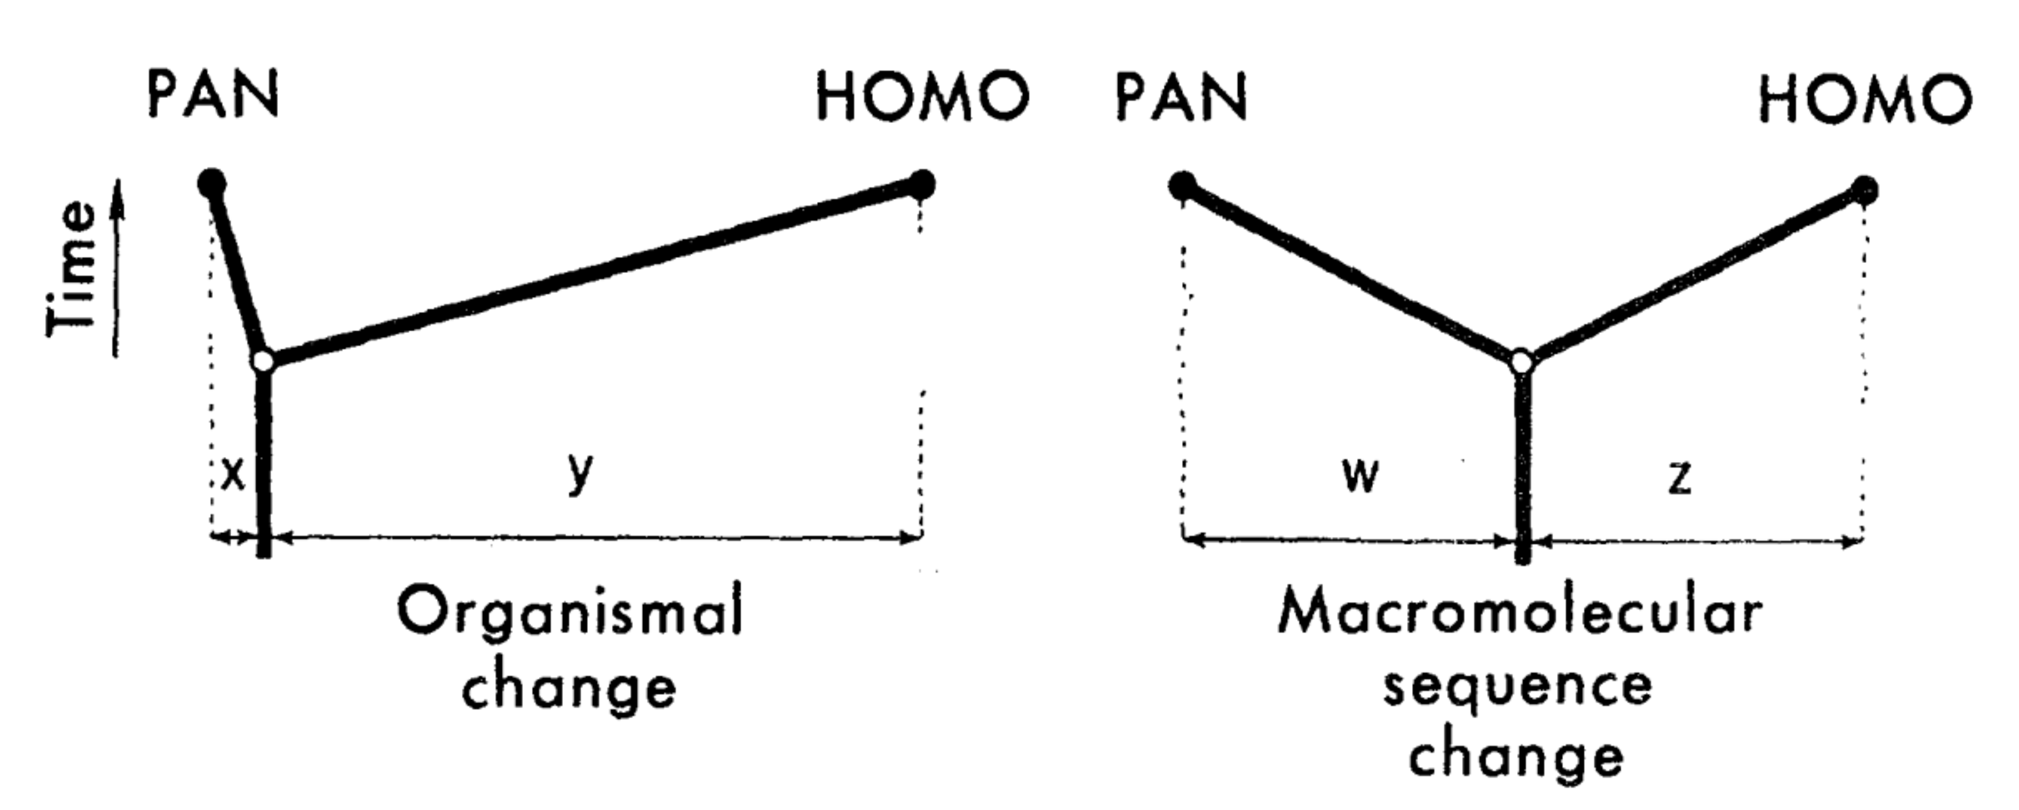
\includegraphics[scale=0.35]{Figs/king_wilson.pdf}
\caption{Schematic diagram of the rates of organismal and molecular
  change in human (Homo) and chimpanzee (Pan). Figure taken from
  \citet{King1975}.}
\label{fig_king_wilson}
\end{figure}

Continued genetic, anatomical and \emph{in situ} study of primates has
somewhat tempered the imbalance in the ``organismal'' rates of human
and chimpanzee evolution as drawn by King and Wilson: the evolution of
human form does not appear to be exceptional within the context of
other mammalian and primate species \citep{Carroll2003}, and humans
variously share and differ in many behavioral and sexual
characteristics with chimpanzee and gorilla
\citep{Harcourt1980,Goodall1986,Vigilant2004}. On the molecular level,
however, few plausible connections between human-specific phenotypes
and molecular changes have been found, lending support to King and
Wilson's 30-year old prediction
\citep{Clark2003,Sequencing2005a,Bradley2008}. In the first comparison
of the human and chimpanzee genomes, \citet{Sequencing2005a} wrote
that ``We thus find minimal evidence of acceleration unique to either
the human or chimpanzee lineage across broad functional categories.''
Still, these general findings do not preclude the possibility of
\emph{some} amount of protein-coding change playing a role in the
differences between humans and our close relatives. Accordingly,
studies of protein-coding evolution in humans and our close relatives
have provided insight into the evolution of the great apes as a whole,
identifying patterns of adaptive evolution or relaxed constraint in
genes related to sound perception \citep{Clark2003}, coloration
\citep{Mundy2007}, language \citep{Enard2002} and brain size
\citep{Montgomery2011}. Adaptive evolution in genes related to sperm
production \citep{Clark2005} and immune defense \citep{Sawyer2005a}
has also repeatedly been found in primates, though these patterns of
selective pressures appear to be shared throughout the mammalian
clade, as evinced in Chapter \ref{ch_mammals2}.

Within this context, the recent sequencing of a western lowland
gorilla genome provided an opportunity to further examine patterns of
molecular evolution within human and our closest living relatives,
even if the power to detect lineage-specific adaptive events (or the
actual presence of such events) was likely to be limited. Previous
phylogenetic estimates indicate that the \ac{hcg} common ancestor
lived 6-10 \ac{myr} ago, with humans and chimpanzees diverging a few
\ac{myr} after that \citep{Bradley2008}. The inclusion of gorilla
within a comparative analysis would thus provide 6-10 \ac{myr} of
additional branch length to the primate tree in addition to allowing
the distinction between substitutions along the \ac{hcg} and the
\ac{hc} ancestral branches of the phylogenetic tree. With gorilla,
potential differences in the molecular evolution of our distant (e.g.,
\ac{hcg}) and more recent (e.g., \ac{hc}) great ape ancestors could be
investigated. Furthermore, analysis of the terminal branch of gorilla
could provide additional information regarding the constancy or
variability of evolutionary rates in the recent evolution of the
\ac{aga} (e.g., human, chimpanzee and gorilla). Previous analyses have
estimated a greater \ac{ne} in chimpanzee compared to human
\citep{Sequencing2005a,Siepel2009a}, and somewhat surprisingly, one
study identified more lineage-specific \acp{psg} in chimpanzee than in
human (\citet{Bakewell2007}, but see \citet{Mallick2009} for evidence
of false positives in these results). Gorilla, representing a third
independent \ac{aga} lineage with a slightly longer branch length than
human and chimpanzee, will provide an important additional data point
in this regard.

In collaboration with Stephen Montgomery and Nick Mundy from the
Zoology department of Cambridge University, I performed an analysis of
the evolution of protein-coding genes in gorilla and the \ac{aga}. The
analysis was jointly designed by Stephen, Nick and myself; all data
collection, calculations and statistical analyses were performed by
me; and results were interpreted by us and other members of the
gorilla analysis consortium. As with the analysis for the \ac{mgp}, a
summary of our main findings was contributed to the manuscript
describing the gorilla genome, which is currently undergoing peer
review. The description of the methods and results presented here is
similar to the text included in the submitted manuscript and
supplementary documents.

The main goal of the analysis was to use codon models of evolution to
identify genes with accelerated \nsyn substitution rates in the
terminal and ancestral branches of the \ac{aga}. To do this, I
collected a highly filtered set of coding alignments in six primate
species (the African great apes plus orangutan, rhesus macaque, and
marmoset) and used a series of \acp{lrt} based on the branch models
implemented in \acp{paml} to identify accelerated genes along branches
of the primate phylogeny. Within the wider context of the gorilla
genome analysis, which included an investigation of \ac{ils} in coding
and non-coding regions, a secondary goal of this study was to identify
patterns of \ac{ils} within and near protein-coding genes. A third
goal was to use the set of genome-wide coding alignments to estimate
lineage-specific average \dnds ratios. Through the connection between
\ac{ne} and \dnds, these results could be used to place gorilla and
the ancestral \ac{aga} branches within the wider context of changing primate population sizes through time \citep{Sequencing2005a}.

\section{Data collection and quality control}
\subsection{Primate one-to-one orthologous genes}

All orthologous gene sets, gene trees, and sequence alignments were
collected from Ensembl Compara release 60 using the Ensembl Perl API
\citep{Vilella2009,Flicek2011}. I first identified the set of genes
sharing one-to-one orthology among all six primates by collecting
homology annotations from the \ens \cmp database: for each human
protein-coding gene, the orthology status for each non-human species
was assigned to different categories based on the number of homologous
genes and the type of homology as annotated by \ens. Homologs were
classified as either one-to-one (e.g., one homolog available and
either an ``ortholog\_one2one'' or ``apparent\_ortholog\_one2one''
homology type), deleted (e.g., no homolog available), duplicated
(e.g., multiple homologs available), or human duplication (e.g., one
homolog available but containing an ``ortholog\_one2many'' annotation,
indicating that there are multiple human homologs for that single
non-human homolog). From an initial set of 20,746 human protein-coding
genes, this procedure identified 12,652 genes with 6-way 1-to-1
orthology; 4,809 genes with primate deletions; 1,171 genes with
primate duplications; 308 genes with human-specific duplications; and
1,806 genes with mixed patterns of duplication and deletion.

%Figure \ref{fig_gorilla_dup_dels} shows two Venn diagrams of shared
%gene deletions and duplications in chimpanzee, gorilla, orangutan and
%macaque relative to the human set of protein-coding genes. The \emph{a
%  priori} expectation, assuming somewhat random ongoing process of
%gene duplication and deletion, was that species most closely related
%to human would contain fewer deletions and duplications relative to
%the human gene set, with increasingly distant species having greater
%numbers. Ignoring the overlap, a comparison of the size of each
%species' circle in Figure \ref{fig_gorilla_dup_dels}A showed this to
%be the case: 2,279 deletions were found for chimpanzee, 2,344 for
%gorilla, 3,050 for orangutan, and 3,015 for macaque (marmoset, not
%shown, had 3,215 deletions). The counts of duplications showed a
%similar pattern, except for a notable excess of gorilla duplications:
%gorilla had 273 duplications relative to human, compared to 74 in
%chimpanzee, 165 in orangutan, 522 in macaque, and 722 in marmoset. The
%excess of duplications in gorilla appeared to be anomalous, and is
%expected to decrease in future refined versions of the gene annotation
%set.

%\begin{figure}
%\centering
%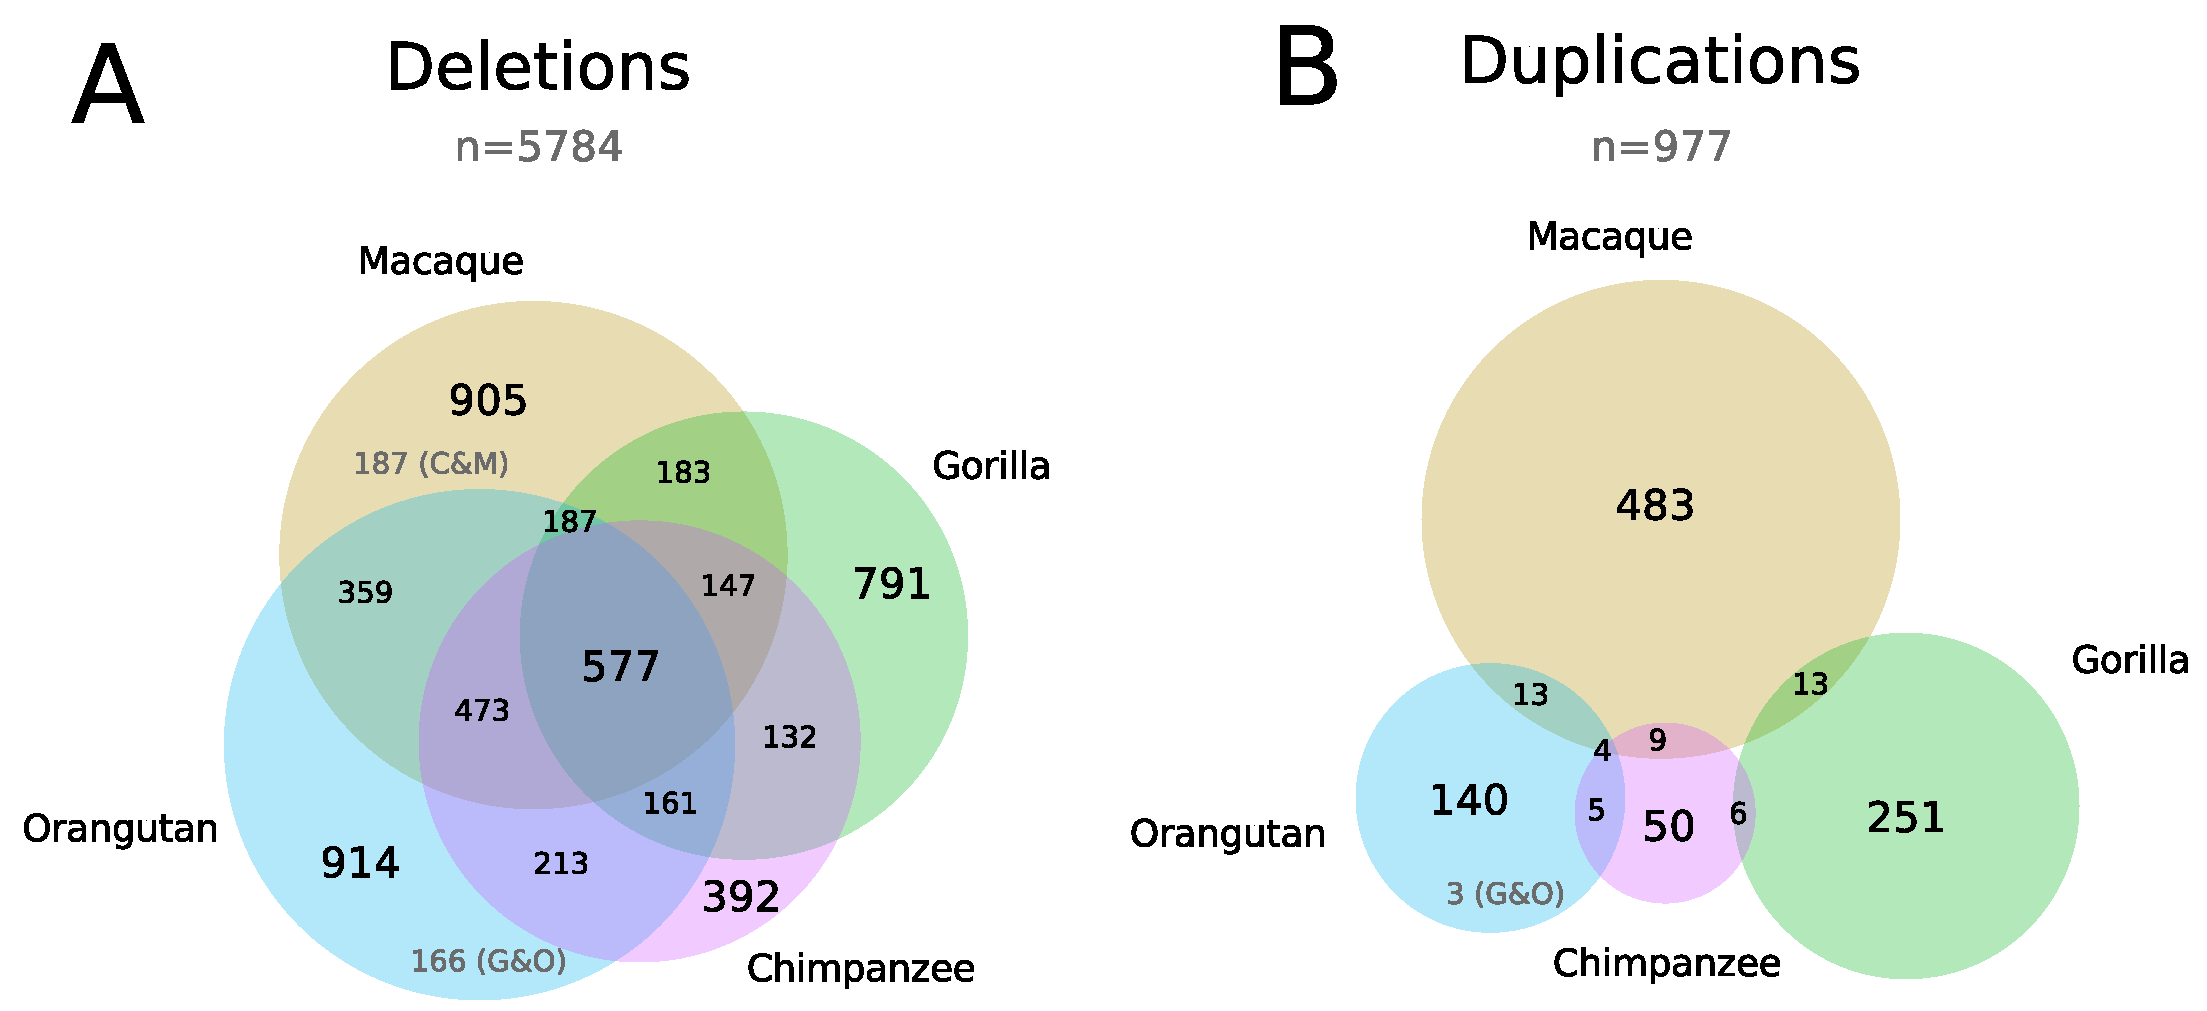
\includegraphics[scale=0.4]{Figs/gorilla_dup_dels.pdf}
%\caption{Venn diagrams of shared and unique (A) deletions and (B)
%  duplications in non-human primates relative to the set of human
%  genes.}
%\label{fig_gorilla_dup_dels}
%\end{figure}

%The amount of overlap between species in the Venn diagrams of Figure
%\ref{fig_gorilla_dup_dels} shows how often deletions and duplications
%relative to human are shared between different primate
%species. Interestingly, deletions appeared to be more often shared
%between two or more species than duplications, suggesting that certain
%genes may be more prone to independent deletion events than
%duplication events. It should be stressed, however, that this analysis
%and view of gene duplications and deletions was not intended to
%rigorously identify gene duplication and deletion events in
%primates. A more appropriate approach would be to explicitly place
%duplication and deletion events along the primate phylogeny using one
%or multiple mammalian outgroups, but these comparisons were made
%mostly to gain an understanding of whether gene deletions or
%duplications were more responsible for genes which did not have
5one-to-one orthology within \ac{aga}.

%\begin{figure}
%\centering
%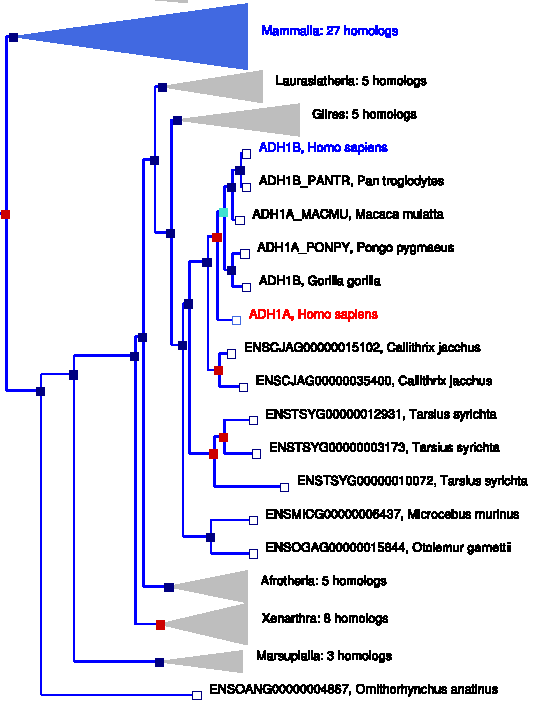
\includegraphics[scale=0.9]{Figs/adh1a.pdf}
%\caption{Part of the inferred gene tree relating the human gene
%  \gene{ADH1A} and its homologs. \gene{ADH1A} is highlighted in red
%  and the human gene \gene{ADH1B} is highlighted in blue. The gene
%  tree data were taken from \ens release 60.}
%\label{fig_adh1a}
%\end{figure}

%Many of the shared deletions in Figure \ref{fig_gorilla_dup_dels} were
%likely the result of recent human duplications where the homology to
%other primate genes was not detected, either due to incorrect
%assembly, missing primate gene annotations or the conservative rules
%used by \ens to assign orthology relationships based on gene trees
%\citep{Vilella2009}. An example is the gene \gene{ADH1A}: although the
%homology annotations indicated the gene as lacking a homolog in all 5
%of the primates included here, a detailed analysis of \gene{ADH} gene
%family evolution identified clear one-to-one orthology between
%\gene{ADH1A} genes within primates \citep{Oota2007}. The authors
%showed that the cluster of \gene{ADH} genes likely arose through
%mammalian-specific and primate-specific duplication events in
%chromosome 4, raising the possibility that these duplicated genomic
%segments could have been falsely collapsed into a single assembled
%sequence in non-human assemblies. The \cmp gene tree for \gene{ADH1A},
%pictured in Figure \ref{fig_adh1a}, shows that some primate species
%are missing annotated \gene{ADH1A} or \gene{ADH1B} orthologs,
%consistent with a collapsed assembly in that region. Perhaps as a
%result of these missing orthologs, the human \gene{ADH1A} is placed as
%an outgroup to the entire clade of \ac{aga} \gene{ADH1} orthologs,
%causing it to be annotated as lacking human orthology in the \ac{aga}
%species. In addition to illustrating the problems involved in
%identifying orthology between highly-duplicated genes in
%closely-related species, this example showed that the \ens one-to-one
%orthology annotations were conservative. The 12,652 one-to-one
%orthologs identified using these annotations were selected for further
%analysis.

\subsection{Collecting and filtering six-way codon alignments for one-to-one genes}
\label{sec_ils_mask}

Codon alignments of all one-to-one orthologs were extracted from the
6-way primate genomic alignments pre-calculated by the \ens pipeline
using the \ac{epo} pipeline \citep{Paten2008a,Paten2008}. I extracted
and concatenated primate alignment blocks corresponding to the
protein-coding portion of each exon from the consensus coding
transcript of each human gene. These alignments were then flattened to
the human reference by removing all columns with insertions in
non-human primates or deletions in the human lineage. Since the
\ac{epo} alignments are generated on the DNA level and the current
evolutionary analysis was to be performed on the codon level, I
clearned each alignment for codon analysis by masking out any triplets
containing stop codons or out-of-frame gaps. Of the original 12,562
one-to-one genes identified above, 11,538 codon alignments were
successfully collected. The reduction numbers came from 1,024 genes
which were discarded because an entire species was missing from that
region of the primate \ac{epo} alignment; the species most often
missing in the alignments were orangutan (520 genes), marmoset (475 genes),
and macaque (328 genes).

The low levels of divergence between the primate species being
analyzed made it extremely important to avoid the inclusion of any
incorrectly-aligned material. The expected number of lineage-specific
substitutions per gene scales linearly with the length of that
species' terminal branch, meaning a small number of sequencing,
assembly or alignment errors causing apparent \nsyn substitutions
along one of the short \ac{aga} terminal lineages could easily lead to
a false positive inference of accelerated evolution. As such, an
aggressive set of filters was applied to each alignment prior to the
\ac{paml} analysis.

First, the chimpanzee, orangutan, macaque and marmoset sequences were
filtered using PHRED or PHRED-like quality scores downloaded from the
UCSC (chimpanzee and macaque) or WUSTL (orantugan and marmoset)
websites. Any bases with a quality score lower than 30 (corresponding
to an expected error rate of 1 in 1000 bases) were replaced with `N's.

An initial analysis of the PHRED filtered 6-way alignments revealed
many stretches of alignment with obviously non-homologous sequence in
one or more non-human genomes. These regions appeared similar to the
clustered substitutions seen in Chapter \ref{ch_mammals1}, although
alternative splicing or mis-annotated genes could be ruled out as a
causative factor since the EPO alignments were built on the DNA level
and only the human transcript structure was used. The most likely
cause was some combination of mis-assembled genomic sequence and
misalignment by the EPO pipeline. I found that genes containing these
dubious aligned stretches were prominent among the initial list of
accelerated genes based on these alignments.

To exclude such regions from analysis, I applied a filter based on
windows of inferred lineage-specific substitutions, using an approach
similar to that described for the filtering of mammalian alignments in
Chapter \ref{ch_mammals1}. First, the codon alignment was analysed
with the codeml program of \ac{paml} v4.14 using a M0 model to infer
substitutions in the terminal lineages of the 6-species tree. Using
the branch lengths (expressed as the expected number of substitutions
per codon) and substitution evens inferred by \ac{paml}, I analyzed
the density of codons containing lineage-specific non-synonymous
substitutions within every 15-codon window along the alignment. Any
window containing more than 10 \nsyn substitutions per codon per unit
of branch length was masked with `N's. After analyzing the preliminary
results from this method, a number of additional heuristic corrections
were made to avoid excess stringency or lenience: first, branch
lengths below 0.05 substitutions per codon were set to 0.05 in order
to avoid too small of a denominator; second, the masking threshold was
decreased from 10 to 5 for any windows overlapping alignment gaps or
ambiguous nucleotides; third, codons containing two or three
nucleotide substitutions along one branch were counted as two \nsyn
substitutions.

This procedure resulted in a total of 72,729 nucleotides being masked
from 1,156 genes, with the following breakdown of the numbers of genes
in which each species had at least one nucleotide masked: 12 human,
195 chimpanzee, 232 gorilla, 296 orangutan, 271 macaque and 324
marmoset.  The low number of genes from which any human sequence was
masked indicated that the filtering was not overly conservative, while
the high numbers in non-human primates indicated that those genomes
are more likely to contain highly localized, apparently spurious runs
of \nsyn substitutions in the regions of EPO alignments corresponding
human transcripts.

A final filter was applied to avoid a potential bias from
substitutions in regions of \ac{ils} between sequences in human,
chimpanzee, and gorilla. \ac{ils} regions are genomic segments where
either gorilla-chimpanzee or gorilla-human share a most recent common
ancestor, deviating from the ``canonical'' relationship where human
and chimpanzee share the most recent ancestor. Roughly 20-30\% of the
genome shows evidence of \ac{ils} within the African great apes
\citep{Hobolth2007}. In cases where a \syn or \nsyn substitution
occurs along the ancestral branch of a genomic segment subject to ILS,
the assumption of a single phylogenetic tree per gene is violated and
\ac{paml} cannot correctly infer a single substitution event. Instead,
two substitutions must be inferred in order to fit the observed site
pattern to the canonical phylogenetic tree. The method can choose to
infer either two identical substitutions (one along each of the
terminal ``ILS'' branches sharing the most recent common ancestor) or
one substitution along the \ac{hcg} ancestral branch and a second
reversion substitution along the non-ILS terminal branch. I observed
that PAML tended to infer the latter sequence of events as the most
likely substitution history. The long length of the \ac{acg} ancestral
branch may have contributed to the two-substitution path being the
most likely one.

Given the high proportion of expected sites under \ac{ils}, I applied
a simple filtering method to mask out codons that were likely the
result of a single substitution in an ancestral \ac{ils} lineage. Any
codon where either gorilla-human or gorilla-chimpanzee shared a codon
sequence that was different from both orangutan and the non-\ac{ils}
species (either human or chimpanzee) was considered likely to contain
an ancestral \ac{ils} substitution. The human, chimpanzee and gorilla
sequences at these sites were all masked with `N's, causing \ac{paml}
to treat those nucleotides as missing data. This resulted in 7,841
codons being masked from 4,340 genes prior to analysis with
\ac{paml}. Although the \ac{ils} masking was relatively widespread
across genes, its effect on the results was conservative with respect
to the number of inferred substitutions, and likely had a minimal
impact on the identification of accelerated genes: the majority of
genes (2,605) contained only one masked codon, which would be unlikely
to seriously attenuate an otherwise strong signal of lineage-specific
acceleration.

\subsection{Manual identification of remaining alignment or assembly errors}

A manual analysis of genes with suspiciously strong evidence for an
accelerated \nsyn substitution rate identified 4 genes with apparent
alignment or assembly error that escaped the various filtering steps
described above. (Note that the \ac{lrt} method designed to test for
lineage-specific acceleration is described in Section
\ref{sec_accel_lrt}.) For each potentially erroneous gene, a manual
analysis of the alignment was undertaken by visually inspecting the
codon alignment, the locations of inferred substitutions, and the
protein-based alignment of the same gene downloaded from v60 of the
\ens \cmp database. In total, 4 genes---\gene{ITPK1}, \gene{POLR2A},
\gene{ATN1}, and \gene{GAS6}---were found to show evidence of serious
misalignment and were removed from further analysis. Two other genes,
\gene{SUPT16H} and \gene{POLR1A}, contained similarly strong signals
of lineage-specific acceleration and elevated numbers of \nsyn and
\syn substitutions. These genes were also manually assessed, but no
obvious signs of misalignment were found. The four genes with clear
errors were removed from the set of genes analyzed for the remainder
of the analysis, resulting in 11,534 total genes analyzed by the
\acp{lrt} described below.


%\gene{ITPK1}, which codes for an inositol triphosphate kinase with 415
%amino acids and had a primate \dnds of 0.094 (as estimated from
%\ac{paml} using the M0 model), showed 28 \nsyn and 10 \syn
%substitutions in the chimpanzee lineage and a strong signal for
%chimpanzee acceleration. The alignment showed few chimpanzee
%substitutions in the first half of the protein, but a high density of
%masked chimpanzee nucleotides and mixed synonymous and \nsyn
%chimpanzee substitutions in the second half. The substitutions that
%were not masked by the window-based filter were presumably just below
%the threshold used. I analyzed the alternative protein-based
%alignments from \ens \cmp, which included a different stretch of
%sequence for the chimpanzee \gene{ITPK1} ortholog in the second half
%of the protein. This sequence had far fewer mismatches, indicating
%that the \ac{epo} genomic alignments from which our data were
%generated contained a chimpanzee misalignment in the latter half of
%the protein.

%\gene{POLR2A}, which codes for the largest subunit of RNA polymerase
%II with 1,971 amino acids and a primate \dnds of 0.043, contained 22
%\nsyn and 70 \syn substitutions in the gorilla lineage and a strong
%signal for gorilla \dn acceleration. The gene showed a highly
%conserved pattern across the bulk of its length, except for the final
%250-300 amino acids which contained a highly repetitive sequence and
%long, dense clusters of substitutions in both gorilla and
%orangutan. The protein-based alignments showed a much cleaner gorilla
%sequence, but stretches of spurious substitutions were instead found
%in the chimpanzee sequence, suggesting that this repetitive region is
%subject to frequent genome assembly and/or alignment error.

%\gene{ATN1} codes for a protein of unknown function which, upon the
%expansion of a trinucleotide repeat within the region, leads to
%dentatorubral pallidoluysian atrophy, a rare neurodegenerative
%disorder \citep{OkamuraOho1999}. With 1,191 amino acids and a
%relatively high primate \dnds of 0.339, \gene{ATN1} showed 105 \nsyn
%and 54 \syn substitutions in gorilla, with a strong signal for
%acceleration. The gorilla substitutions were evenly interspersed along
%the length of the gene, but they were noticeably absent from the first
%and last 100 amino acids. Gorilla also showed a long 50-amino acid gap
%prior to the high-substitution region. A comparison to the
%protein-based alignments did not show a different gorilla sequence;
%rather, it contained a chimpanzee sequence with a similar pattern of
%high numbers of substitutions. This suggested that there may be a
%duplicated or pseudogenic version of the gene region in primates which
%contains many substitutions relative to the \gene{ATN1} gene. Thus, it
%was likely that the pattern of gorilla substitutions seen in the
%\gene{ATN1} alignment was not indicative of substitutions acting on a
%functional ortholog of human \gene{ATN1}. 

%\gene{GAS6} codes for a protein thought to be involved in the
%stimulation of cell proliferation. It contains 722 amino acids, has a
%primate \dnds of 0.150, and contained 29 \nsyn and 8 \nsyn gorilla
%substitutions and yielded a strong signal for gorilla
%acceleration. Manual analysis of the alignment revealed a block of
%\nsyn substitutions in the middle of the gene directly adjacent to a
%block of sites which were masked by the window-based filter. The
%protein-based alignments contained a different gorilla sequence in the
%concerned region, but this different sequence contained a
%qualitatively similar number of differences relative to human.

\section{Codon model evolutionary analysis}

The set of evolutionary models and \acp{lrt} used to identify
accelerated genes in the 6-way primate alignments were designed by
Stephen Montgomery, Nick Mundy and myself.

\begin{figure}
\centering
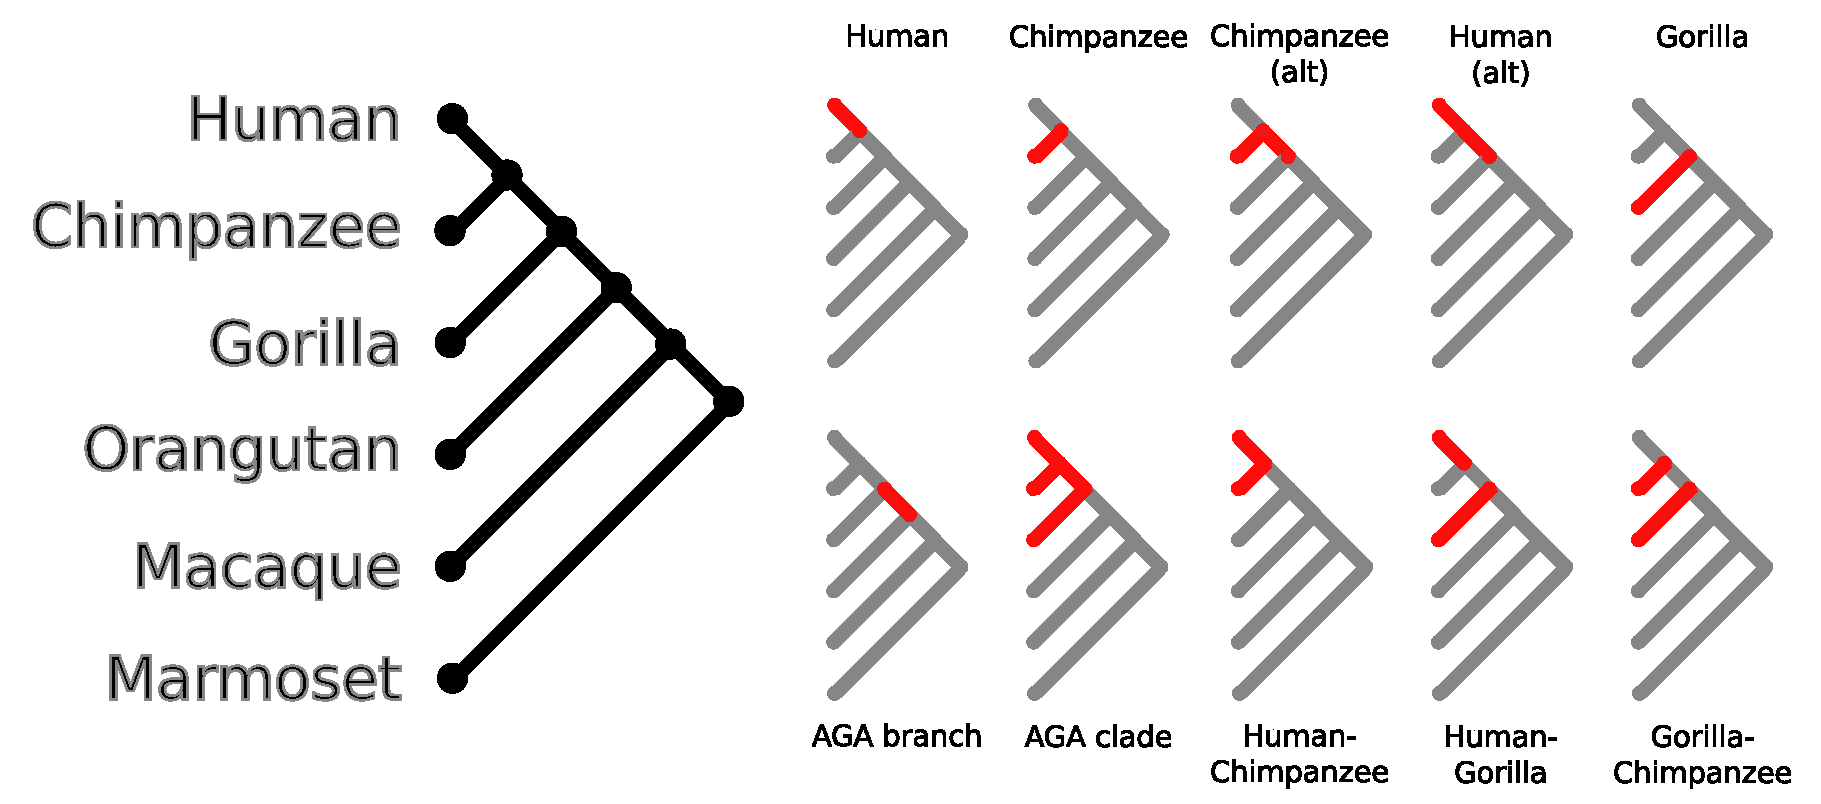
\includegraphics[scale=0.5]{Figs/gorilla_branch_models.pdf}
\caption{Branch models used to construct \ac{lrt} for detecting
  accelerated genes in various branches of the \ac{aga} phylogeny. The
  foreground branches for each model are highlighted in red. The label
  above or below each tree describes which species or group of species
  is under investigation with each model. AGA---African great apes;
  alt.---alternative model.}
\label{fig_gorilla_branch_models}
\end{figure}

To detect signals of accelerated and decelerated evolution in gorilla
and the \ac{aga}, a total of 10 so-called branch models of evolution
were specified. Each branch model separates the phylogenetic tree into
two categories of branches, foreground and background branches, which
are then modeled as evolving with separate \dnds ratios by including
distinct foreground and background \omg parameters in the model
\citep{Yang1998,Yang1998a}. Figure \ref{fig_gorilla_branch_models}
shows the models used in this study, with background branches in gray
and foreground branches in red. Each branch model was designed to
allow for an elevated (accelerated) or decreased (decelerated) \dnds
ratio in a branches of particluar interest to the study of \ac{aga}
evolution. \ac{paml} was used to estimate parameters and calculate the
likelihood value for each model in Figure
\ref{fig_gorilla_branch_models} applied to each coding alignment. A
\ac{lrt} was performed for each model by comparing the likelihood of
the alignment under that branch model to the likelihood of the
alignment under the simpler M0 model, which uses a single \omg
parameter for the entire tree. This test will be referred to as a
branch-LRT to distinguish it from the more commonly used branch-site
LRT described below. The branch-LRT statistic represents the strength
of evidence that a given branch model is a better fit than the simpler
M0 model to a given alignment; in other words, a large statistic can
be interpreted as an indication that the evolution of the gene is
well-explained by different \dnds ratios in the foreground and
background branches of the tree. The \ac{ml} estimate of the two \omg
parameters could be used to identify genes where the estimated
foreground \omg was higher or lower than the background. Genes where
the foreground \omg was higher than the background were categorized as
accelerations, and genes where the foreground \omg was lower than the
background were categorized as decelerations. Using the \ac{lrt}
statistic and the distinction between accelerations and decelerations,
a signed \ac{lrt} statistic was constructed for each branch-LRT, where
accelerated genes were assigned the branch-LRT statistic and
decelerated genes were assigned the negative of the branch-LRT
statistic. In this way, a single number was used to encapsulate the
direction and strength of evidence in support of a shifted \dnds ratio
in the foreground branch of each model presented in Figure
\ref{fig_gorilla_branch_models}.

A highly positive signed branch-LRT score represented strong evidence
for a lineage-specific elevated \dnds ratio. Such an elevated ratio
could be explained either by positive selection or relaxed constraint
\citep{Nielsen2005,Sequencing2005a}. To attempt to distinguish the
former from the latter, I used the branch-site \ac{lrt} implemented in
\ac{paml} \citep{Zhang2005} to identify genes with significant
evidence for positive selection acting along a branch or
clade. Similar to the branch-LRT, the branch-site LRT requires a
predefined separation of branches into foreground and background
categories. However, the branch-site LRT is specifically tuned towards
identifying temporally and spatially localized episodes of positive
selection \citep{Nielsen1998,Yang2002b,Zhang2005}. The branch-site LRT
was run for the Human, Chimpanzee, Gorilla, AGA branch and AGA blade
models shown in Figure \ref{fig_gorilla_branch_models}.

For each model tested, the full length codon alignment was input to
the \texttt{codeml} program from the \ac{paml} package along with a
phylogenetic tree corresponding to the accepted species tree structure
(the labeled tree in Figure \ref{fig_gorilla_branch_models}). The
`cleandata’ option was set to 0 (e.g., alignment columns containing
gaps were not removed from the analysis but were treated as ambiguous
data), and branch lengths inferred by \texttt{codeml} based on the
initial M0 model model analysis were used as the initial branch
lengths for all other models tested.

When the null model of evolution in the branch-LRT is true, the
ac{lrt} statistic---measured as twice the difference in log-likelihood
values between the branch model and the null M0 model---should be
distributed according to a \chisq distribution with one degree of
freedom. The same null distribution was assumed for the branch-site
LRT. Strictly speaking, the branch-site LRT null distribution should
be a 50:50 mixture of a point mass at 0 and \chisq with one degree of
freedom, but the more conservative \chisq distribution is recommended
by Ziheng Yang to guard against violations of model assumptions
\citep{Yang2007}. \pvs for each branch-LRT and branch-site LRT result
were thus calculated by comparing the absolute value of the \ac{lrt}
statistic to a chi-squared distribution with 1 degree of freedom. The
Benjamini-Hochberg method \citep{Benjamini1995} was used to correct
for multiple testing within each branch model by controlling the
\ac{fdr}.

The ``alternative'' models shown in Figure
\ref{fig_gorilla_branch_models}, which were designed to detect
accelerations along the human and chimpanzee lineages while correcting
for the difference in branch length between the human-chimpanzee
terminal branches and the gorilla terminal branch, did not yield
significantly different results from the equivalent uncorrected
models, so results from those tests were discarded from the rest of
the analysis.

\subsection{Branch-LRT and branch-site LRT results}

\begin{table}
\centering \scriptsize
\begin{tabular}{lrrrrrr}
\toprule
 & \multicolumn{2}{c}{Acceleration} & \multicolumn{2}{c}{Deceleration} & \multicolumn{2}{c}{Branch-site LRT} \\
Model / Species & $p<0.05$ & FDR$<0.1$ & $p<0.05$ & FDR$<0.1$ & $p<0.05$ & FDR$<0.1$ \\
  \midrule

\input{Tables/gorilla_lrt_results.txt}
\bottomrule
\end{tabular}
\caption{Branch-LRT and branch-site LRT results. Each row corresponds
  to a model in Figure \ref{fig_gorilla_branch_models}, except for the
  two ``alternative'' models, which were excluded from the
  analysis. Each cell represents the number of genes for which the
  \ac{lrt} was significant at the specified threshold for the given
  model. \pvs were calculated by comparing the \ac{lrt} statistic to a
  \chisq distribution with one degree of freedom. The \acf{fdr} was
  controlled within each model separately for the branch-LRTs and for
  the branch-site LRTs using the \citet{Benjamini1995} method.}
\label{table_gorilla_lrt_results}
\end{table}

Table \ref{table_gorilla_lrt_results} presents for each model, and at
two significance thresholds ($p<0.05$ and LRT$<0.1$), the number of
significantly accelerated and decelerated genes according to the
branch-LRT and the number of positively-selected genes according to
the branch-site LRT. The number of $p<0.05$ accelerated genes for
almost all of the branch models was greater than the expected number
under the null model. Assuming equivalent amounts of acceleration and
deceleration, the expected number of $p<0.05$ accelerations and
decelerations using the branch LRT would be roughly
$11,538\times0.05/2=288$ genes. All models showed an excess of
accelerated genes, with between 300 and 873 genes accelerated at the
nominal $p<0.05$ threshold. Significant evidence for deceleration, was
found at levels equal to or slightly below the null expectation, with
between 151 and 314 decelerations per model. The ``AGA Branch'' model
showed a notable tendency towards lower \dnds ratios, with the fewest
accelerations (300) and most decelerations (314) out of all models
tested.

Looking at strongly accelerated or decelerated genes, defined as those
corresponding to $FDR<0.1$, roughly equivalent numbers were found in
the three terminal lineage models (human / chimpanzee / gorilla) with
between 10-19 strong accelerations and between 1-2 strong
decelerations for each model. The other models were much more
variable, possibly due to differences in power resulting from
different foreground branch lengths, with the AGA Clade model showing
many strongly-shifted genes (56 strong accelerations and 9 strong
decelerations) and the AGA Stem model showing very few (3 strong
accelerations and 1 strong deceleration). The Human-Chimpanzee,
Gorilla-Human, and Gorilla-Chimpanzee models, designed to detect
evidence for parallel accelerations and decelerations, showed roughly
twice as many strongly accelerated and decelerated genes as their
terminal-branch counterparts (29-45 strong accelerations and 3-6
strong decelerations), as might be expected based on the doubled
amount of branch length in the foreground portions of their models.

\section{Parallel accelerations}
\label{sec_parallel_accel}

I used the linaege-specific gene acceleration LRT results to evaluate
the prevalence and strength of parallel gene accelerations between
\ac{gh}, \ac{gc}, and \ac{ch} during the time period since the
speciation of each pair. Parallel accelerations where analyzed on
three levels: first, quantifying genome-wide signals for shared gene
acceleration; second, identifying \ac{go} terms enriched for shared
accelerations; and third, identifying genes with the strongest
evidence of parallel accelerations for each species pair.

A suitable statistic by which to measure the amount of evidence for
parallel accelerations was first developed. Three of the branch models
shown in Figure \ref{fig_gorilla_branch_models} were designed to be
sensitive to parallel accelerations in the species pairs of interest
(e.g. the models labeled ``Human-Chimpanzee'', ``Human-Gorilla'', and
``Gorilla-Chimpanzee''), but I found that many of the strongest
branch-LRT results for these three models were driven by \nsyn
substitutions in primarily one of the two species pairs. For example,
\gene{SUPT16H}, the gene with the highest branch-LRT under the
``Human-Gorilla'', yielded a LRT score of 51.14. However, it appears
that most of this signal was due to substitutions in the gorilla
lineage: looking at the lineage-specific human and gorilla \ac{lrt}
values for the same gene, I found a gorilla LRT of 61.1 and a human
LRT of -1.34 (where a negative value indicated an estimated decrease
in \dnds relative to the background branches). Thus, human and gorilla
clearl did not both experience independently accelerated \dnds levels
in \gene{SUPT16H}, despite the strong LRT result from the
gorilla-human branch model. For this reason, LRT results from these
three ``parallel'' branch models were excluded from further
analysis. To ensure that genes identified as undergoing parallel
acceleration showed independent evidence in each lineage of having
experienced \dnds accelerations, I instead used the minimum of both
lineages' independent branch model LRT value as the statistic for
parallel acceleration in each pair of species. This statistic will be
referred to as \lrtmin. The counts of parallel accelerations and
decelerations shown in Table \ref{table_gorilla_lrt_results} were
calculated using the \lrtmin statistic for accelerations and an
equivalent LRT$_{max}$ statistic for decelerations (as the signed
\ac{lrt} statistic was negative for decelerated genes).

\subsection{Genome-wide rates of shared acceleration}

A randomized resampling strategy was used to determine whether the
number of parallel accelerations at a given branch-LRT cutoff
threshold was significantly greater than that expected given
independent distribution of each species' accelerated genes. For each
iteration of the randomization, a set of pseudo-``accelerated'' genes
for each paired species was chosen by randomly sampling $N_{acc}$
genes (where $N_{acc}$ is the number of observed lineage-specific
accelerations for each species at the given LRT cutoff threshold) from
among the 11,534 total genes. The number of overlapping accelerated
genes was counted at each iteration, and the fraction of iterations
which yielded a greater number of overlapping accelerations than the
observed number of parallel accelerations was taken as the \pv for the
significance of the observed number of overlapping accelerations at
the given cutoff threshold. This was repeated for each species pair,
and for cutoff thresholds ranging from 0 to 5.

The magnitude of over- or under-representation of parallel
accelerations was also estimated by calculating the co-occurrence
excess (defined as $N_{obs}/N_{exp} - 1$) of accelerated genes for
each pair of species and the same range of branch-LRT cutoff
thresholds. The expected number of parallel accelerations was
calculated using the same null expectation as the randomization test:
that each lineage has a proportion of accelerated genes, and that the
accelerations for each lineage are independently distributed amongst
the 11,534 total genes. The expected fraction of overlapping
accelerated genes is thus the product of each lineage's proportion of
accelerated genes, and $N_{exp}=N_{accA}/N\times N_{accB}/N\times N$
where $N$ is the total number of genes and $N_{accA}$ and $N_{accB}$
are the numbers of accelerated genes in each lineage. For each species
pair and cutoff threshold, one hundred bootstrap replicate datasets
were sampled from the 11,534 genes. The co-occurrence excess was
calculated for each replicate, and confidence intervals were
calculated at the 50\% level from the set of bootstrap values.

\begin{figure}
\centering
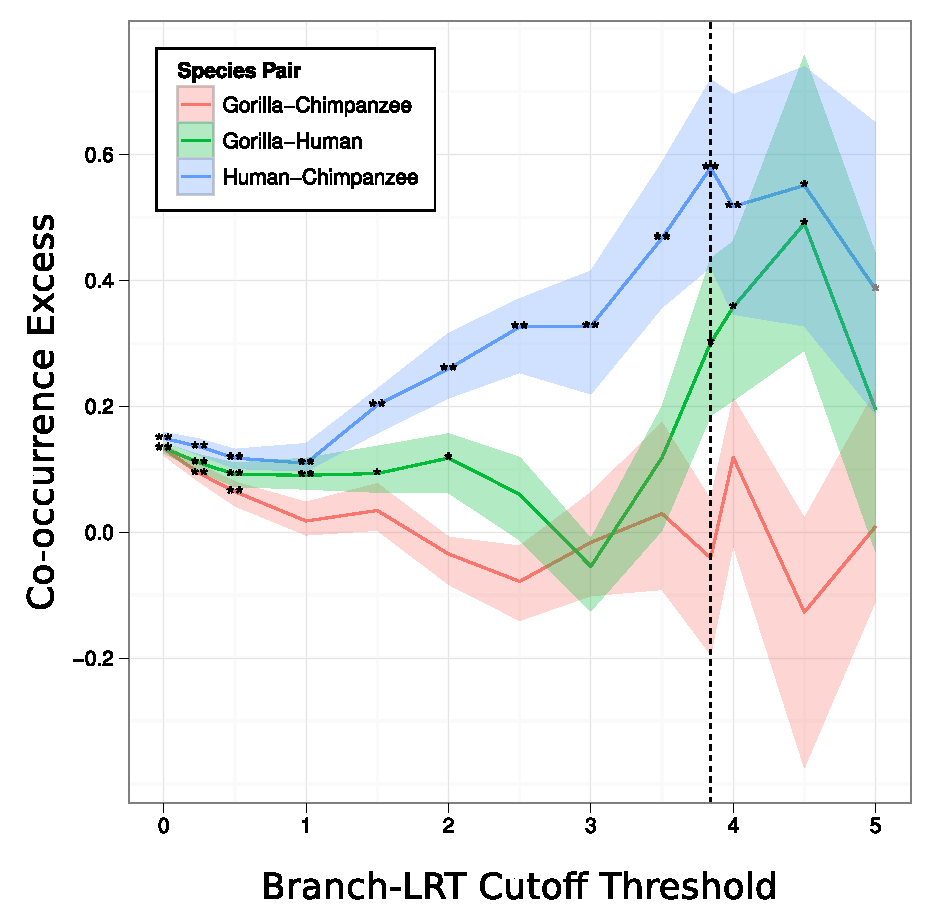
\includegraphics[scale=0.7]{Figs/gorilla_parallel.pdf}
\caption{Genome-wide excess of parallel accelerations in pairs of
  \ac{aga} species at various LRT cutoff values. Parallel gene
  accelerations in three species pairs (Gorilla-Chimpanzee, red;
  Gorilla-Human, green; Human-Chimpanzee, blue) were identified using
  branch model LRT cutoffs from 0 to 5 (x-axis; see text for details
  on how parallel accelerations were identified), and the
  co-occurrence excess between lineage-specific and parallel
  accelerations at each LRT cutoff was calculated (y-axis; the 50\%
  bootstrap confidence interval is shaded). A randomization procedure
  was used to identify significant enrichment for parallel
  accelerations: two black stars indicate $p<0.01$, one black star
  indicates $p<0.05$, and one gray star indicates $p<0.1$ for the
  given species pair and LRT cutoff. A vertical dotted line indicates
  the LRT cutoff corresponding to the 95\% chi-squared significance
  value.}
\label{fig_gorilla_parallel}
\end{figure}

The results of the randomisation test and co-occurrence calculations
are shown in Figure \ref{fig_gorilla_parallel}. For each species pair,
the co-occurrence excess is plotted as a function of the LRT cutoff
threshold with a solid line drawn at the co-occurrence value and a
shaded area drawn around the 50\% bootstrap confidence interval. The
results of the randomization test are indicated by one or two stars
drawn adjacent to the co-occurrence value for the given dataset. For
reference, a dotted vertical line is drawn at the LRT cutoff
corresponding to a nominal $p<0.05$ \chisq cutoff value. At lower
(i.e. more lenient) LRT cutoff values a greater number of genes in
each of the paired species were accelerated, and at higher (i.e. more
stringent) LRT cutoff values fewer genes are accelerated. This sample
size effect can be seen in the wider confidence intervals and larger
amounts of apparent stochastic noise at higher LRT cutoffs.

A trend was clear when comparing the co-occurrence excess levels and
randomisation test \pvs between the \ac{gh}, \ac{gc} and \ac{hc}
species pairs: \ac{hc} showed the largest excess of parallel
accelerations, \ac{gh} showed an intermediate amount of excess, and
\ac{gc} showed the least excess. This trend was consistent across a
wide range of threshold cutoff values and was supported by both the
co-occurrence excess values and the results of the randomisation
tests. The \ac{hc} species pair showed randomisation $p<0.01$ for all
but the two highest (i.e., most stringent) threshold cutoffs and a
maximum co-occurrence excess of nearly 60\%. The \ac{gh} species pair
showed significantly enriched acceleration overlap at $p<0.05$ for
threshold cutoffs below 2 and at 3.84, 4 and 4.5. The \ac{gh}
co-occurrence excess was noticeably lower than that of \ac{ch}, but
above zero for all but one threshold cutoff. The \ac{gc} species pair
showed little evidence of genome-wide enrichment for parallel
accelerations, with a significant overlap only at weak threshold
cutoffs of 0.5 or below and a co-occurrence excess hovering around
zero across the range of cutoff thresholds.

That the \ac{hc} pair showed the largest number of overlapping
accelerations was not entirely surprising, as human and chimpanzee
share the most recent speciation event among the three species
pairs. Thus, they presumably share the greatest number of
environmental and behavioral traits that might have caused a gene to
experience increased \nsyn substitutions in both lineages. More
interesting was the difference in overlap levels between the \ac{gc}
and \ac{gh} species pairs. Whereas the \ac{gc} pair showed little
genome-wide evidence for excess parallel acceleration, the \ac{gh}
pair showed a slight but consistent signal for more parallel
accelerations than expected by chance. This could be due either to a
greater degree of biological or environmental similarity in \ac{gh}
compared to \ac{gc}, or it could be the result of some underlying bias
in the data, such as differences between human and chimpanzee in
population size or genome quality.

\subsection{\ac{go} terms enriched in shared accelerated genes}

The second approach used to characterize genes with parallel
accelerations was to identify \ac{go} terms enriched for genes with
evidence for parallel acceleration in each pair of \ac{aga}
species. The methodology used to identify enriched \ac{go} terms will
be described Section \ref{sec_gorilla_go}, but the parallel results
are described here for clarity.

For each species pair, genes with \lrtmin$>1.5$ were considered
significant in the \ac{go} enrichment tests. This more lenient
threshold was used, since few genes were independently accelerated at
the 95\% chi-squared threshold of 3.84 in both lineages (25 genes for
\ac{gc}, 40 for \ac{gh}, and 51 for \ac{hc}; Table
\ref{table_gorilla_lrt_results}). At a \lrtmin threshold of 1.5, the
\ac{gc} pair yielded 206 accelerated genes, \ac{gh} yielded 238, and
\ac{hc} yielded 286. The sections of Table \ref{table_gorilla_go}
labeled ``Human-Chimpanzee Parallel'', ``Gorilla-Chimpanzee Parallel''
and ``Gorilla-Human Parallel'' show the terms most enriched for
parallel accelerations.

Although no species pair yielded \ac{go} terms significantly enriched
after correction for multiple testing, a number of terms were enriched
at a nominal $p<0.05$ significance using \ac{fet}. The top three terms
for \ac{hc} parallel accelerations were ``neuropeptide signaling
pathway'', ``regulation of DNA-dependent transcription'' and
``microtubule-based movement''; for \ac{gc} parallel accelerations,
``protein autophosphorylation'', ``innear ear development and positive
regulation of transcription factor activity''; and for \ac{gh}
parallel accelerations, ``Wnt receptor signaling pathway'', ``sensory
perception of sound'' and ``skeletal system morphogenesis'' showed
some enrichment for significant genes.

\begin{landscape}
\centering \scriptsize
\begin{longtable}{rrrllrrrrl}
\toprule

Ann. & Sig. & Exp. & ID & Definition & \ac{fet} & \topgo & \goseq &
Len. & Top 5 Significant Genes \\
\endhead

\\
\multicolumn{6}{l}{\normalsize{Table \ref{table_gorilla_go}} (\emph{continued on next page})} & & & & \\
\endfoot

\\[-1.8ex] \hline \hline
\endlastfoot

\midrule
\multicolumn{4}{l}{Human} & & & & & & \\
\midrule
\input{Tables/gorilla_go_1.txt}

\midrule
\multicolumn{4}{l}{Chimpanzee} & & & & & & \\
\midrule
\input{Tables/gorilla_go_2.txt}

\midrule
\multicolumn{4}{l}{Gorilla} & & & & & & \\
\midrule
\input{Tables/gorilla_go_3.txt}

\midrule
\multicolumn{4}{l}{Human-Chimpanzee Parallel} & & & & & & \\
\midrule
\input{Tables/gorilla_go_4.txt}

\midrule
\multicolumn{4}{l}{Gorilla-Chimpanzee Parallel} & & & & & & \\
\midrule
\input{Tables/gorilla_go_5.txt}

\midrule
\multicolumn{4}{l}{Gorilla-Human Parallel} & & & & & & \\
\midrule
\input{Tables/gorilla_go_6.txt}

\midrule
\multicolumn{4}{l}{\ac{aga} Branch} & & & & & & \\
\midrule
\input{Tables/gorilla_go_7.txt}

\midrule
\multicolumn{4}{l}{\ac{aga} Clade} & & & & & & \\
\midrule
\input{Tables/gorilla_go_8.txt}

\bottomrule
\caption{\ac{go} terms enriched for lineage-specific or parallel
  accelerated genes. All terms with \ac{fet} $p<0.05$ are shown sorted
  by their \topgo \pv. Non-significant \pvs from the \topgo
  \citep{Alexa2006a} and \goseq \citep{Young2010a} methods, which
  account for the \ac{go} ontology structure and gene length bias,
  respectively, are shown in gray. The 5 most strongly accelerated
  genes within each category are included for illustrative
  purposes. Ann.---the number of genes annotated with a given term;
  Sig.---the number of significant genes annotated with the term;
  Exp.---the number of significant genes expected given independent
  association between significant genes and \ac{go} terms; Len.---the
  mean length of genes annotated with the term.}
\label{table_gorilla_go}
\end{longtable}
\end{landscape}


Interestingly, the term ``sensory perception of sound'' was enriched
at $p<0.05$ in all three species pairs, but only three genes
(\gene{LOXHD1}, \gene{CDH23} and \gene{GPR98}) were significant at
\lrtmin$>1.5$ in all three pairs; all other significant genes were
unique to each species pair. The sound perception genes which were
uniquely significant in the \ac{gh} pair were \gene{EYA1},
\gene{USH1C}, \gene{MYO3A} and \gene{SLC1AC}; for the GC pair,
\gene{OTOF} and \gene{FZD4}; and for the HC pair, \gene{DIAPH1},
\gene{MYCBPAP} and \gene{DFNB31}. This suggested that the tendency of
genes involved in sound perception to experience midly to moderately
elevated \dnds levels was relatively widespread in all three \ac{aga}
genomes, with variation in the specific genes having undergone
acceleration in each species or species pair. It is also worth noting
that the enrichment for this term among parallel accelerated genes was
strongest in the \ac{GH} species pair, where the enrichment was
significant at $p<0.05$ in both the \topgo and \goseq tests. The term
had $p>0.05$ for those tests in the \ac{gc} and \ac{hc} pairs,
indicating that human and gorilla share a slightly stronger signal for
parallel accelerated evolution in hearing genes than do the other
pairs of \ac{aga} species.

\subsection{Top parallel accelerated genes}

The third method of analysis was a survey of the top parallel
accelerated genes for each species pair and for all three species
using the same \lrtmin statistic described above. Table
\ref{table_gorilla_top_genes} (located in Appendix \ref{ch_lrts} at
the end of this thesis) shows the top 10 accelerated and
positively-selected genes for a variety of \ac{aga} lineages and
tests; the top parallel accelerations according to the \lrtmin
statistic can be found towards the bottom of Table
\ref{table_gorilla_top_genes}.

Among the top genes accelerated across all three lineages are
\gene{LOXHD1}, a gene comprised of PLAT domains which was recently
shown to be necessary for auditory hair cell function
\citep{Edvardson2011}; \gene{ITIH3}, a plasma serine protease
inhibitor potentially involved in prevention of tumor metastasis and
associated with risk of myocardial infarction \citep{Ebana2007}; and
\gene{PARP3}, a member of the ADP ribosyl transferase family which has
recently been characterized as playing a role in telomeric stability,
response to DNA damage, and neural crest development
\citep{Rouleau2011,Boehler2011}. The molecular and medical evidence
for the functional activity of these genes suggests that the elevated
\dnds levels across all three African great apes are not well
explained by a substantial loss of functional constraint; other
possible causes might be relaxed evolutionary constraint due to a
decreased effective population size relative to the primate
background, positive selection due to functional adaptation, or some
combination of the two. 

\section{\acf{go} term enrichments}
\label{sec_gorilla_go}

Gene ontology (GO) term annotations for the ``biological process''
ontology tree were downloaded from release 60 of the Ensembl human
database \citep{Flicek2011} and assigned to the alignment
corresponding to each human gene. Three complementary methods were
used to assign \pvs for \ac{go} term enrichment among the most
accelerated genes for each branch-LRT performed and genes with
evidence of parallel acceleration in a pair of species. For
lineage-specific accelerations, the 95\% \chisq cutoff value of the
branch-LRT was used to identify accelerated genes. Parallel
accelerations for each species pair were identified by genes with a
minimum branch-LRT value of 1.5 in both species of interest (more
detail on the analysis of parallel accelerations is included in
Section \ref{sec_parallel_accel}).

The first test was a standard one-tailed \ac{fet} applied to the 2x2
contingency table of significant / non-significant genes which were
annotated / not-annotated with a given \ac{go} term. The second
method, implemented in the \topgo program \citep{Alexa2006a}, is also
based on the \ac{fet} statistic but additionally compensates for the
structure of the GO hierarchy by iterating through the directed
acyclic graph and removing nodes from consideration when certain
descendant nodes have already shown significant enrichment (see
\citet{Alexa2006a} for complete details of the algorithm). The main
effect of the \topgo algorithm is to identify and remove semantically
repetitive terms (e.g., terms that are nearby in the \ac{go} ontology
and are annotated with similar sets of genes) from the set of most
significantly enriched results by reducing the \pvs of terms with more
highly-enriched neighboring terms. The third method, implemented in
the \texttt{goseq} program \citep{Young2010a}, accounts for a
potential gene length bias in the propensity for a gene to yield a
significant LRT results. As the sequence length can have a strong
impact on the significance of \ac{lrt} results \citep{Anisimova2001}
and some \ac{go} terms tend to contain longer genes
\citep{Young2010a}, I found it important to correct for this when
identifying enriched terms. The \goseq program first uses the set of
gene-wise \pvs and gene lengths to fit a smoothed \ac{pwf} which
predicts the expected proportion of significant accelerations given a
gene’s length. This \ac{pwf} is then used to adjust the identification
of significantly-enriched \ac{go} terms to correct for potential
over-representation of terms with significantly longer or shorter mean
gene lengths. Although the \goseq program was designed primarily for
the functional analysis of RNA-seq data (where gene length bias is a
widely-acknowledged confounding factor) I found it to be effective in
identifying potentially misleading \ac{go} enrichment results for the
current analysis.

The results of the GO enrichment analysis are summarized in Table
\ref{table_gorilla_go}. For each branch model (or pair of species for
parallel accelerations), all terms with a \ac{fet} over-representation
$p<0.05$ and 5 or more significant genes are shown sorted by their
\topgo p-value. Any \topgo or \goseq \pvs above $p=0.05$ are colored
gray instead of black. Terms with non-significant \topgo \pvs are
likely to have a closely-related term with stronger enrichment higher
in the list, while terms with non-significant \goseq \pvs should be
treated with caution due to a detected length bias in the detection of
accelerated genes.

It is worth noting that none of the \ac{go} term enrichments for any
of the branch-LRTs shown in Table \ref{table_gorilla_go} remained
significant at \ac{fdr}$<0.1$ after applying the \citet{Benjamini1995}
correction (results not shown). The lack of significance after
correcting for multiple tests could be taken as evidence that no
strong associations between accelerated genes and \ac{go} terms
existed in these results. However, it may also be due to a variety of
other factors, including limited power of branch models to detect
\dnds shifts, noise in the \ac{go} annotation of genes, or the
specific choice of LRT cutoffs used to identify significant
accelerations. Other studies have avoided the use of cutoff thresholds
by using different tests such as the Mann-Whitney U test to identify
terms with a significantly lower distribution of \pvs than expected
\citep{Clark2003,Kosiol2008}, but this was not done here. Despite the
lack of strongly-controlled statistical significance, the use of a
nominal $p<0.05$ cutoff to identify enriched GO terms for display in
Table \ref{table_gorilla_go} yielded a limited set of enriched terms
for each branch-LRT that summarized the strongest functional
associations with moderately to strongly accelerated genes.

\begin{landscape}
\centering \scriptsize
\rowcolors{1}{white}{gray!10}
\begin{longtable}{lllllllb{6cm}}
%\begin{longtable}{>{\raggedright}b{1.8cm}>{\raggedright}b{1cm}>{\raggedright}b{1cm}>{\raggedright}b{1.2cm}>{\raggedright}b{1cm}>{\raggedright}b{.9cm}>{\raggedright}b{.9cm}>{\raggedright}b{8cm}lll}

\toprule
Study & FG Species & Gene Count & Test & Ontology & Accel. & \acp{psg} & Top 5 enriched terms \\
\midrule
\endhead

\midrule
\\
\multicolumn{8}{l}{\normalsize{Table \ref{table_gorilla_studies}} (\emph{continued on next page})} \\
\endfoot

\\[-1.8ex] \hline \hline
\endlastfoot

\input{Tables/gorilla_studies.txt}

\bottomrule

\caption{A comparison of previous genome-wide studies of primate gene
  evolution. Nine studies of positive selection or accelerated \dnds
  in primates, including the current study, are summarized by various
  factors including the number of genes analyzed, the tests of
  selection performed, the accelerated or positively-selected gene
  count, and the most strongly enriched functional terms. The current
  results were largely consistent with previous results in the
  percentage of accelerated and positively-selected genes
  identified. In contrast, the functional terms detected as enriched
  for accelerated genes varied widely, both within the set of
  previously-published studies and with the current results.}
\label{table_gorilla_studies}

\end{longtable}
\end{landscape}

\section{Comparison with previous genome-wide scans for accelerated or positively-selected genes}

A number of studies have previously investigated the prevalence and
functional associations of \acp{psg} and genes with elevated \dnds in
primate genomes, often using branch-LRTs or branch-site LRTs similar
to those used here. Although these studies have varied widely in the
exact datasets and analytical methods employed, a qualitative and
quantitative comparison their main results helped to appreciate the
variability of previously published genome-wide results in
primates. Table \ref{table_gorilla_studies} presents a summary of
results from the current analysis plus 8 previous genome-wide scans
for accelerated or positively-selected genes. This table was
originally compiled by Stephen Montgomery for the gorilla consortium,
but it has been heavily modified and condensed into the current form.

The proportion of accelerated genes detected using branch-LRT methods
(or close equivalents) ranged from 7.07\% to 20.24\%; results from the
current study, which ranged from 4.64\% in chimpanzee to 5.75\% in
human, was only slightly lower than the typical range of
previously-published values. For the proportion of genes experiencing
positive selection under the branch-site \ac{lrt} (or similar), the
current results results (ranging from 1.23\% in human to 1.66\% in
gorilla) again fell within the lower end of the the published range of
0.43\% to 8.72\%. Most published studies did not show a large
difference in the proportion of accelerated or positively-selected
genes between chimpanzees and humans; our results further confirm this
trend and extend to gorilla the observed conistency in numbers of
lineage-specific accelerated and positively-selected genes between
different \ac{aga} species.

Table \ref{table_gorilla_studies} highlights the wide range of
biological functions and processes that have commonly been found
enriched for genes subject to accelerated evolution or positive
selection. Terms involving immune functions, olfaction, and amino acid
metabolism have most commonly been identified. The GO term enrichments
based on the current branch-LRT results did not recover many terms in
common previous studies. This may be the result of a different type of
sensitivity in the specific branch-\acp{lrt} used here, where gene
accelerations in \ac{aga} lineages \emph{relative to the primate
  background rate} were detected, as opposed to high rates of
evolution on their own. For example, immune genes with high \dnds
ratios across all primates were not likely to be identified as
accelerated in this study, since immune genes tend to be subject to
positive selection throughout the mammalian phylogeny as opposed to
one particular lineage or another (see Chapter
\ref{ch_mammals2}). This could explain the lack of any apparent immune
enrichment in the current results.

Interestingly, the \ac{go} term ``sensory perception of sound'' was
among the top enriched terms in both the gorilla lineage and
gorilla-human parallel accelerated genes. Although previous studies
have detected enrichment for olfaction and visual perception
\citep{Clark2003,Nielsen2005,Macaque2007}, this appears to be the
first genome-wide analysis to provide strong evidence for an abundance
of genes involving sound perception to have been subject to elevated
\dnds ratios in the \ac{aga}. Some evidence was also found for
enrichment of brain-related terms in human and gorilla, including
``brain development'' (Gorilla $p=0.038$, Table
\ref{table_gorilla_go}) and ``nervous system development'' (Human
$p=0.032$, Table \ref{table_gorilla_go}), although both terms may be
subject to a gene length bias and fail to reach $p<0.05$ using the
\goseq method for detecting enriched terms.

%\section{Levels of \acf{ils} within and near genes}

%The close proximity of the \ac{hc} and \ac{hc}-G speciation events
%makes \ac{ils} a prominent feature of the genomic relationship between
%human, chimpanzee and gorilla. Regions showing \ac{ils} should not be
%subject to any particular functional constraint, but the \ac{ne} in
%the great ape ancestor is expected to affect the prevalence of ILS,
%causing less ILS in regions of lower ancestral \ac{ne}
%\citep{Hobolth2011}. Strong purifying selection on genes tends to
%reduce the \ac{ne} within and nearby exonic regions due to background
%selection \citep{Charlesworth1993}, so I sought to characterize the
%effect of the strength of purifying selection, as measured by the
%\dnds ratio in the 6-way primate alignments, on the prevalence of
%\ac{ils} within and around protein-coding regions.

%I first looked at patterns of \ac{ils} density within protein-coding
%genes. I separated the 11,534 one-to-one genes into five equally-sized
%\dnds bins, using the \dnds ratios estimated by \ac{paml} using the
%one-ratio M0 model and the filtered 6-way coding alignments. Before
%performing the \ac{ils} masking step described in Section
%\ref{sec_ils_mask}, each alignment site of each gene was assigned a
%substitution pattern according to a comparison of the human,
%chimpanzee and gorilla nucleotides and the orangutan nucleotide. A `1'
%indicated similarity and a `0' indicated dissimilarity to the
%orangutan nucleotide, and for each site a binary ``site pattern'' was
%given by concatenating the values in the order of human, chimpanzee
%and gorilla. Thus, a site where human and gorilla matched the
%orangutan sequence but chimpanzee was different was denoted \texttt{010}. I
%counted and stored the total number of sites with each pattern for
%each gene, skipping all sites with a gap or ambiguous nucleotide in
%any species.

%The most important patterns allowing for discrimination of \ac{ils}
%versus non-\ac{ils} sites are \texttt{110} (a likely substitution in the
%\ac{hc} ancestor), \texttt{101} (a likely substitution in a HG \ac{ils}
%ancestor), and \texttt{011} (a likely substitution in a GC \ac{ils}
%ancestor). Due to the scarcity of substitutions along the short
%ancestral branch, I identified genes with strong evidence of \ac{ils}
%by requiring the presence of more \ac{ils} patterns than non-\ac{ils}
%patterns within a gene---specifically, when $n_{101} + n_{011}$ was
%greater than $n_{110}$. A total of 1,974 genes (17.1\%) showed
%evidence of \ac{ils} at this threshold, which corresponded well with
%the results of the CoalHMM \citep{Hobolth2007} analysis (performed by
%other members of the analysis consortium) where \ac{ils} was inferred
%at 20\% of gene-coding sites.

%\begin{figure}
%\centering
%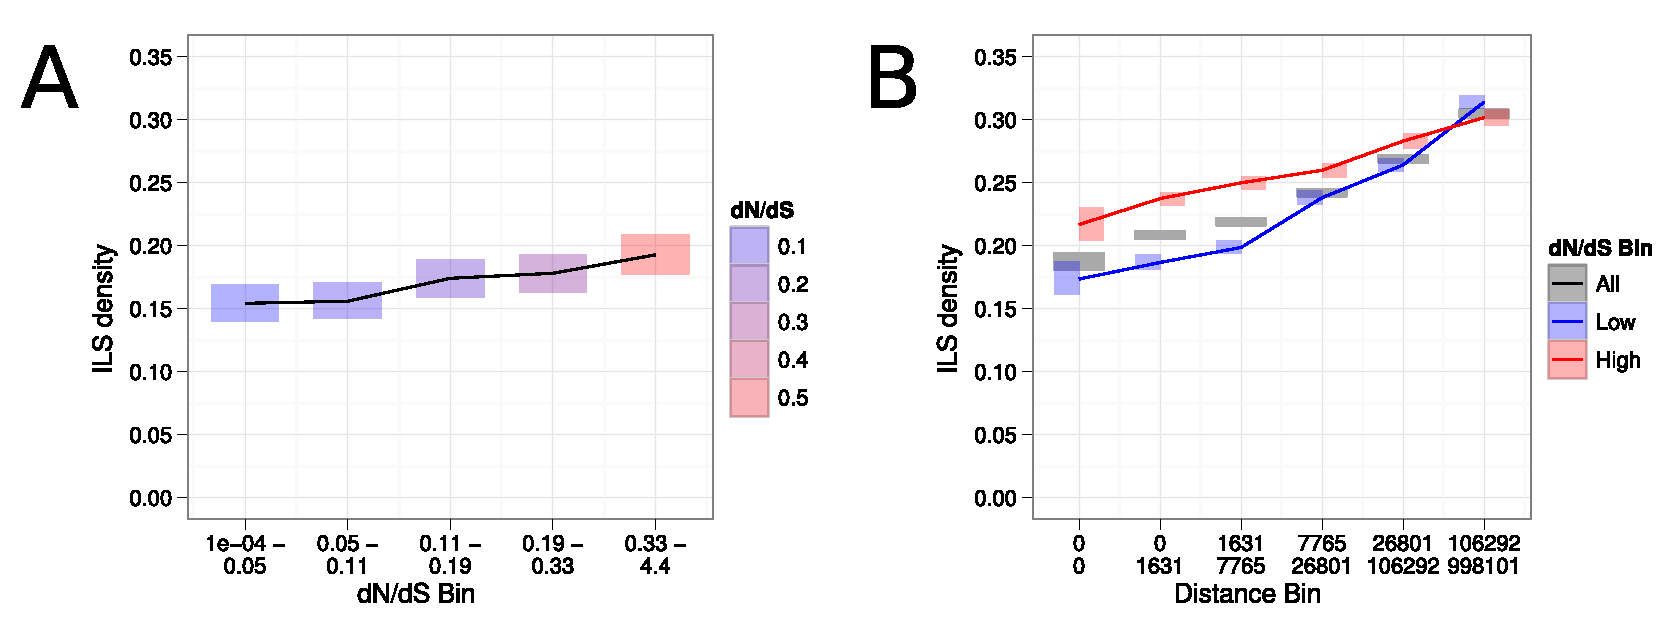
\includegraphics[scale=0.55]{Figs/gorilla_ils.pdf}
%\caption{ILS patterns within and surrounding genes. (A) Genes were
%  separated into five equally-sized \dnds bins and the fraction of
%  genes with strong evidence of \ac{ils} was calculated for each
%  bin. The black line is drawn at the fraction of \ac{ils} genes, and
%  the high and low points of each block corresponds to the 95\%
%  confidence interval. Genes with lower \dnds values contained
%  significantly lower amounts of \ac{ils}, showing the influence of
%  long-term purifying selection on the ancestral \ac{ne}. (B)
%  Overlapping 10kb windows of primate genomic alignments were analyzed
%  for sites showing patterns of \ac{ils}, and the fraction of 10kb
%  windows with strong evidence for \ac{ils} was calculated. Blocks
%  correspond to 95\% confidence intervals. Black, alignments near all
 % genes; red, alignments near genes with high \dnds values; blue,
%  alignments near genes with low \dnds values. Windows near
%  protein-coding exons showed significantly lower amounts of \ac{ils},
%  with the strongest effect being in regions near genes under strong
%  purifying selection.}
%\label{fig_gorilla_ils}
%\end{figure}

%To estimate the correlation between \ac{ils} prevalence and purifying
%constraint in genes, I used the \ac{ils} site patterns and the
%identification threshold described above to calculate the fraction of
%genes with evidence for \ac{ils} within each \dnds bin. A 95\%
%confidence interval was calculated for each \dnds bin based on 1000
%non-parametric bootstrap replicates across genes. Figure
%\ref{fig_gorilla_ils}A shows the result of this analysis, revealing a
%slight but distinct correlation between \ac{ils} density and the
%strength of purifying constraint, with the \ac{ils} density ranging
%from 16\% in genes with the lowest primate \dnds to 19\% in genes with
%the highest \dnds. This was consistent with the expectation that
%\ac{ils} is depleted from regions subject to purifying selection due
%to persistent background selection and a locally decreased \ac{ne}.

%I used a similar approach to investigate the effect of \dnds levels on
%\ac{ils} density in regions surrounding protein-coding genes. First,
%counts of \ac{ils} and non-\ac{ils} patterns were collected for
%segments of Ensembl’s 6-way primate \ac{epo} alignments corresponding
%to 10kb windows of the human genome spaced at 3.3kb intervals,
%yielding 470,344 individual alignment regions. The proximity of each
%region to a protein-coding gene was calculated as the distance from
%the region's center point to the nearest human protein-coding exon. (
%(A distance of zero was assigned if the region's center point was
%within an exon). The identity and \dnds value of the gene containing
%the nearest exon was also stored. Each 10kb region was then identified
%as \ac{ils} or non-\ac{ils} based on which type of site pattern was
%more frequent within that region, as above. Regions were then
%separated into equally-sized bins based on their distance to the
%nearest exon (with a separate bin for windows with a distance of
%zero), and the density of \ac{ils} regions within each bin was
%calculated. Figure \ref{fig_gorilla_ils}B shows the resulting
%proportion of \ac{ils} regions, binned by distance to the nearest
%gene.

%A total of 24.8\% of windows across all distance bins were classified
%as having evidence of \ac{ils}. The same calculations were then
%repeated for windows whose nearest gene was in the lowest 25\%
%quantile (\dnds$<0.05$; Figure \ref{fig_gorilla_ils}B, blue bars and
%line) and in the highest 25\% quantile (\dnds$>0.24$; Figure
%\ref{fig_gorilla_ils}B, red bars and line). The effect of background
%selection on gene-flanking regions of the genome could be clearly seen
%in the reduced \ac{ils} density in windows near to exons; furthermore,
%this effect scaled with the strength of purifying selection on a given
%gene and could be observed in windows further than 100kb from the
%nearest exon.

\section{Genome-wide \dnds ratios in the \ac{aga} phylogeny}

The gorilla genome also provided an opportunity to examine global
trends in the evolutionary dynamics of the African great apes and
their ancestral populations. I used the genome-wide set of coding
alignments to examine lineage-specific \dnds estimates across the
six-primate phylogenetic tree.

Two broad categories of methods have commonly been employed to
estimate ancestral \ac{ne} from comparative genomics data: methods
based on estimating the variance of species divergence times or tree
topologies in samples of coding or noncoding DNA, and methods based on
estimating lineage-specific \dnds ratios in protein-coding genes.

Over the past two decades a number of groups have applied methods
based on the first approach (using variance in divergence times / tree
topologies) to the estimation of primate ancestral populations
(\citet{Takahata1997,Chen2001,Holbolth2007,Burgess2008}; reviewed in
\citet{Siepel2009a}). Despite significant differences in the inference
methods and sizes of datasets used, most analyses were in agreement
that the \ac{ne} of ancestral hominoids was considerably larger than
that found in most present-day populations. However, no consensus
appears to have emerged regarding the absolute \acp{ne} of primate
ancestral populations, and the precision of estimates has been lacking
\citep{Siepel2009a}.

The second general approach is based on comparing lineage-specific
\dnds values estimated from a large amount of aligned protein-coding
sequence. Theory predicts that larger populations should exhibit, on
average, lower \dnds values due to increased efficacy of purifying
selection \citep{Ellegren2008}, and results from several genome-wide
analyses consistently confirmed this trend
\citep{LindbladToh2005Genome,Macaque2007,Sequencing2005a,Warren2008b,Kosiol2008}. All
of these studies were based on alignments of orthologous genes in at
least human and mouse (in addition to other species), and in every
case human had a higher mean \dnds value than mouse. This was
consistent with the theory, given the expectation based on ecological
studies of a much large \ac{ne} in mouse compared to human
\citep{Ellegren2008}. Furthermore, \citet{Ellegren2008} identified a
strong negative correlation between the lineage-specific \dnds
estimates from \citet{Kosiol2008} and the log-\ac{ne} as estimated
from polymorphism data. Within primates, all of the above studies
which included macaque showed it to have a lower \dnds than human and
chimpanzee. There does exist some disagreement regarding the relative
\dnds of human and chimpanzee, however: \citet{Macaque2007} found a
mean \dnds of 0.175 for chimpanzee and 0.169 for humans, while
\citet{Kosiol2008} found a mean \dnds of 0.245 for chimpanzee and
0.249 for humans. While the two values are very similar in both cases,
this discrepancy indicates some remaining uncertainty regarding the
\ac{ne} of humans and chimpanzees since their divergence event 4-6
\ac{myr} ago. Furthermore, the association between sequencing and
assembly errors and inflated estimates of positive selection
\citep{Schneider2009} suggests that lower-quality genomes may be prone
to increased \dnds estimates as a result of such errors, especially in
closely-related primate genomes.

I used \ac{paml} to estimate genome-wide \dnds levels for each branch
in the six-species primate phylogeny from the 11,534 aligned 1-to-1
orthologous genes assembled here. Two alignments were created: an
unfiltered alignment, created by concatenating the alignment of each
gene after sequences were filtered for sequence quality but before the
window-based filter for clustered \nsyn substitutions and the filter
for \ac{ils}-patterned substitutions were applied; and a filtered
alignment, created by concatenating the final alignment of each gene
that was used for the branch-LRT analysis. Both alignments were 7.263
million codons in length. Before being input to \ac{paml}, all columns
containing a gap character or `N' in any species were removed. As
expected, more columns were removed from the filtered alignment due to
additional `N's from the window-based masking procedure: the final
unfiltered alignment contained 5.91 million codons and the final
filtered alignment contained 5.89 million codons. A single \dnds ratio
was first estimated for each alignment using the M0 codon model,
yielding 0.220 for the unfiltered and 0.218 for the filtered
alignment. Separate \dnds values for each branch were then estimated
from each alignment using the free-ratios model implemented in
\ac{paml} (parameter \texttt{model=1}). Because \ac{paml} estimates
parameters based on an unrooted tree using reversible models of
evolution, any estimates of \dnds on the outermost branch (i.e., the
branch connecting the H/C/G/O/M ancestor to marmoset) were ambiguous
as to whether they occurred on the branch leading to marmoset or the
branch leading to the other primates; thus, marmoset was considered an
outgroup in this analysis.

\begin{figure}
\centering
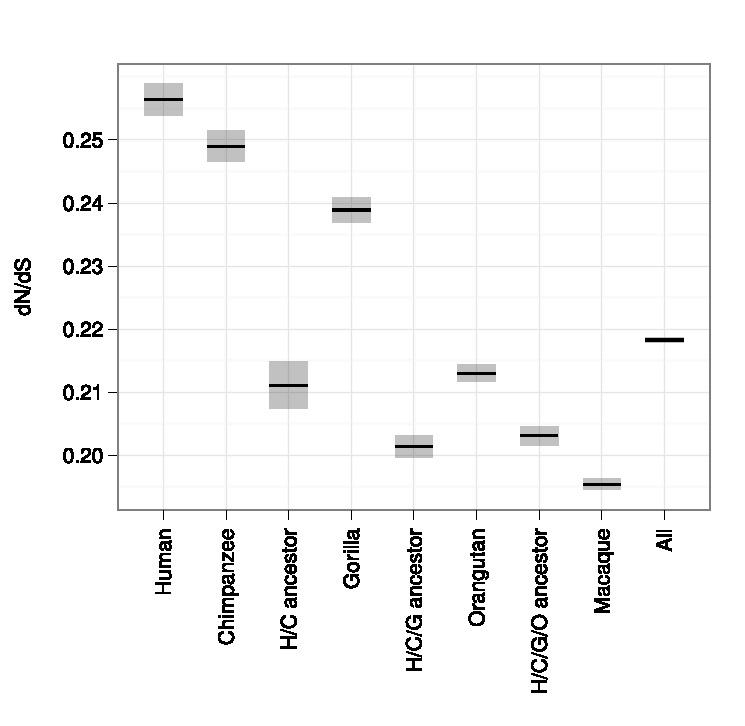
\includegraphics[scale=0.8]{Figs/gorilla_dnds.pdf}
\caption{Genome-wide \dnds values in 5 primate species and their
  ancestral lineages. \dnds ratios were estimated from concatenated
  alignments of 1-to-1 orthologs from six primate species using the
  free-ratios model in \ac{paml}. The most distant aligned species,
  marmoset, was used as an outgroup. Each estimated \dnds ratio is
  plotted as a horizontal line surrounded by a gray box corresponding
  to the standard error estimated by \ac{paml}. Ancestral lineages are
  labeled with the first characters of their descendant species.}
\label{fig_gorilla_dnds}
\end{figure}

\begin{table}
\centering \scriptsize
\begin{tabular}{lrrrrrr}
\toprule
 & \multicolumn{3}{c}{Filtered} & \multicolumn{2}{c}{Unfiltered} & \% \dnds change \\
\cmidrule(r){2-4} \cmidrule(r){5-6}
Branch & \ds & \dnds & S.E. & \dnds & S.E. & (unfiltered vs. filtered) \\
  \midrule

\input{Tables/gorilla_dnds.txt}
\bottomrule
\end{tabular}
\caption{Genome-wide \ds and \dnds values in 5 primate species and
  their ancestral lineages. \dnds ratios were estimated from
  concatenated alignments of 1-to-1 orthologs from six primate species
  using the free-ratios model in \ac{paml}. The unfiltered alignments
  were collected before clustered \nsyn substitutions and sites with
  \ac{ils} patterns were removed. The most distant aligned species,
  marmoset, was used as an outgroup. Ancestral lineages are labeled
  with the first characters of their descendant species. The M0 model
  was used to estimate values for the row labeled
  ``All''. S.E.---standard error of the \dnds ratio estimate
  calculated by \ac{paml}.}
\label{table_gorilla_dnds}
\end{table}

The resulting genome-wide estimates of \ds and \dnds for each branch
are given in Table \ref{table_gorilla_dnds} and plotted in Figure
\ref{fig_gorilla_dnds}. I found that human had a slightly but
significantly higher overall \dnds than both chimpanzee and gorilla
(\dnds$=$0.256, 0.249, 0.239, respectively) and that orangutan,
macaque, and the ancestral lineages all had lower overall \dnds values
than the terminal \ac{aga} branches, ranging from 0.195 for macaque to
0.211 for the human-chimpanzee ancestor. These results were in strong
agreement with equivalent estimates from \citet{Kosiol2008}, who found
overall \dnds values of 0.249, 0.245, and 0.191 for human, chimpanzee,
and macaque, respectively.

A comparison of the global \dnds values from the unfiltered versus the
filtered alignments in Table \ref{table_gorilla_dnds} revealed that
the unfiltered alignments generally yielded higher \dnds values, but
the magnitude of change varied dramatically between branches. The
human terminal branch and all of the ancestral branches showed less
than a 1\% decrease in \dnds as a result of the alignment filtering,
while chimpanzee, gorilla, orangutan, and macaque all showed greater
than 1\% decrease in \dnds. Since the window-based masking procedure
was only applied to clusters of substitutions inf the terminal
branches, the lack of change in \dnds ratios along the ancestral
branches was expected. The smaller magnitude of change in human
(0.39\%) compared to the other extant primate genomes (ranging from
1.03\% to 4.18\%) indicated that the filtering procedure resulted in
far more \nsyn substitutions being removed from non-human sequences
than from human. Interestingly, the magnitude of the \dnds change for
non-human terminal branches appeared to correlate negatively with the
\ds of that branch. Gorilla and chimpanzee, with \ds$=0.0077$ and
\ds$=0.0055$ respectively, both had a $\sim$4\% shift; orangutan, with
\ds=$0.016$, had a $\sim$2\% shift; and macaque, with \ds$=0.032$, had
a $\sim$1\% shift. These observations were consistent with the trend
expected if each genome contained a similar number of erroneous or
misaligned bases, as the larger number of true \nsyn and \syn
substitutions species with longer terminal branch lengths would tend
to ``dilute out'' the signal of elevated \dnds resulting from
misaligned bases. In sum, the comparison between filtered and
unfiltered \dnds levels provided further validation of the use of the
window-based substitution filter. The application of the filter hardly
affected the estimated \dnds ratio of the finished-quality human
genome, but it resulted in branch-length dependent decreases in \dnds
in the lower-quality nonhuman primate genome assemblies. Notably,
chimpanzee showed a marginally higher \dnds than human in the
unfiltered alignment and a significantly lower \dnds than human in the
filtered alignment.

An additional consideration in the interpretation of global \dnds
values was that genes are evolutionarily heterogeneous entities, with
each gene composed of sites evolving under different amounts of
purifying and positive selection due to varying functional and
biological constraints \citep{Whelan2008}. The genome-wide \dnds
estimates in Table \ref{table_gorilla_dnds} were obtained using the
free-ratios codon model, with one \dnds ratio per branch but a
constant \dnds across all alignment sites. Each \dnds ratio estimated
under this model could thus be considered an ``average'' value,
resulting from the combination of sites under strongly purifying,
slightly purifying, neutral and positive selection into a single
alignment. 

This averaging across genes and sites causes two problems for
comparative studies: first, the comparison of genome-wide \dnds values
from different studies is difficult, as the specific genes chosen for
analysis can have a significant impact on the overall results
\citep{Ellegren2008}. Second, the inclusion of sites with very
different selective pressures might decrease the resolution with which
lineage-specific differences in \dnds (and thus \ac{ne}) could be
detected. This is because some fraction of protein-coding sites may
evolve neutrally or under positive selection. Neutrally-evolving sites
in genes should show no relationship with \ac{ne}, and positive
selection should show the opposite effect, with higher \dnds values
with large \ac{ne} due to increased efficacy of positive
selection. Although the proportion of such sites is likely small, they
may obscure the connection between \dnds and \ac{ne}.

One way to better understand the effect of heterogeneously evolving
sites on genome-wide \dnds analyses was to separate out sites with
different selective pressures and analyze each group independently. I
took this approach by separating protein-coding sites into bins based
on their estimated sitewise selective pressure across mammals and
separately analyzing the set of sites within each bin. Sitewise
selection pressures were estimated from all 11,534 genes by applying
\ac{slr} \citep{Massingham2005} to a coding alignment of all Eutherian
orthologs from the Ensembl Compara database. The protein-based MCoffee
alignments calculated by the \ens pipeline were used directly. The \sw
\ac{lrt} statistic calculated by SLR was used to sort all sites by
their strength of evidence for non-neutral selection, with strongly
purifying sites receiving low values, neutral sites receiving
intermediate values, and positively-selected sites receiving high
values. Sites were then split into five bins corresponding to the
following cumulative percentiles of the LRT statistic: 0--0.05,
0.05--0.33, 0.33--0.67, 0.67--0.98, and 0.98--1.0. These ranges were
chosen so that three bins of roughly equal size covered the bulk of
sites, while two bins focused on the 5\% most strongly purifying sites
and the 2\% of sites with strongest evidence for positive
selection. All sites from each bin were concatenated into one
alignment and analyzed with the \ac{paml} free-ratios model as
described above.

\begin{figure}
\centering
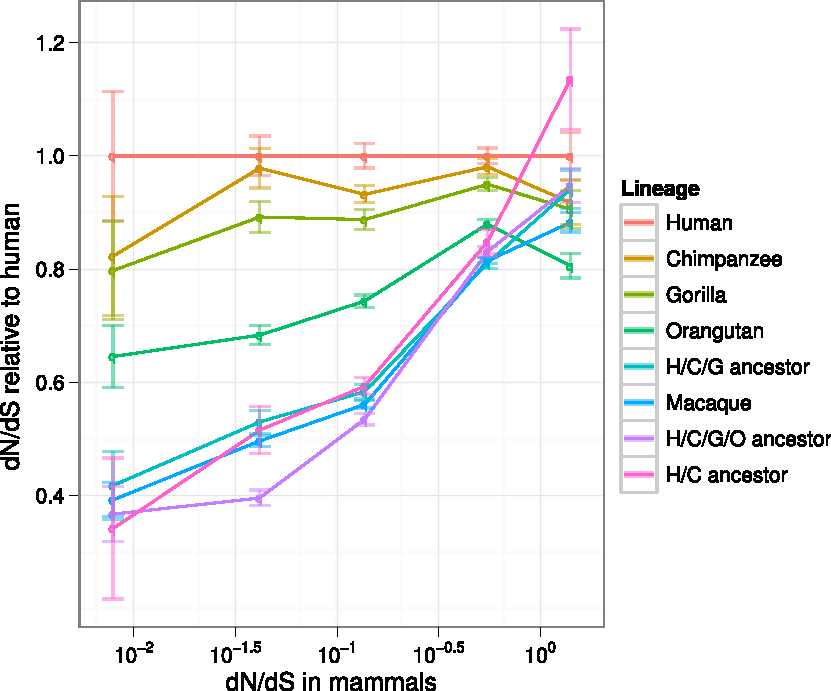
\includegraphics[scale=0.9]{Figs/gorilla_dnds2.pdf}
\caption{Genome-wide branch-specific \dnds ratios in 6-way primate
  alignments binned by \sw selection pressure. Alignment sites were
  sorted by the \sw selection pressure estimated by \ac{slr} in
  mammals, assigned to one of five bins (more details in text),
  concatenated within each bin, and analyzed with \ac{paml} using the
  free-ratios codon model. Estimated \dnds ratios are plotted with the
  human \dnds for each bin on the x-axis and the \dnds for each branch
  (expressed as a fraction relative to the human \dnds in that bin) on
  the y-axis. Lines are drawn connecting estimates from the same
  branch in different bins, and standard errors reported by \ac{paml}
  are shown with error bars. Note the log scale on the x-axis.}
\label{fig_gorilla_dnds2}
\end{figure}

The lineage-specific \dnds ratios estimated from alignments binned by
\sw mammalian selective pressure are shown in Figure
\ref{fig_gorilla_dnds2}. Results from each bin are spread across the
x-axis, and the \dnds ratio for each branch is plotted on the y-axis
as a fraction relative to the human \dnds in that bin.

The 4 lowest \dnds bins showed the same general trends in \dnds levels
as the combined analysis: with human, chimpanzee, and gorilla yielded
the highest \dnds values, followed by orangutan, and finally a cluster
of macaque and the ancestral lineages contained the lowest \dnds
ratios. The H/C/G/O ancestral lineage appeared to have evolved with a
slightly lower \dnds than the other ancestral lineages, though this
difference was only apparent in the 2nd and 3rd bins.

Moving from bins with lower human \dnds to bins with higher human
\dnds, there was a distinct trend across all lineages towards
increased \dnds values relative to human. In the second-lowest bin,
where human had a \dnds ratio of $\sim$0.05, the \dnds difference
between lineages was much stronger than in the second-highest bin,
where human had a \dnds ratio of $\sim$0.55. This trend was consistent
with the expected decrease in the differential effects of \ac{ne} in
sites subject to weaker purifying (e.g., more nearly neutral)
selection.

The pattern of \dnds levels in the highest bin---representing the top
2\% of alignment sites ordered by the LRT statistic, and thus the 2\%
of sites with the greatest site-specific evidence for positive
selection across Eutherian mammals---was distinct from the other 4
bins and warrants further mention. The human \dnds in this bin was
$\sim$1.4, confirming that this subset of alignment sites did indeed
contain a number of sites subject to positive selection. Most of the
terminal and ancestral branches showed a continuation within this bin
of the general trend of increasingly similar \dnds estimates between
lineages, with values for most branches clustered to around
$\sim$88\%--95\% of the human \dnds. However, the \ac{hc} ancestral
lineage showed strikingly increased \dnds values in the highest bin,
and the orangutan branch showed strikingly decreased values. Whereas
the \ac{hc} branch was at $\sim$85\% of the human value in the 4th
bin, its value was $\sim$110\% that of human in the highest bin. In
contrast, orangutan went from $\sim$90\% in the 4th bin to $\sim$80\%
in the highest bin. Such a strong deviation from the consistent trends
observed in the other lineages and other bins suggested that some
effect other than a difference in \ac{ne} may have caused an increase
or decrease in the prevalence of \nsyn substitutions at sites with
evidence for positive selection across Eutherian mammals.
%One approach to
%investigating this artifact more deeply would be to identify the
%subset(s) of genes which contribute most strongly to these lineages’
%deviations from the trend.

\section{Conclusions}

With a comprehensive stage set by previous comparative genome-wide
analyses focusing more closely-related \citep{Sequencing2005a} and
more distantly-related \citep{Macaque2007,Locke2011} primates, the
goal of this study was to investigate

Continued study of the evolution of these candidate parallel
accelerated genes, particularly with attention paid to the recent
population structure of the African great ape species, will further
elucidate the shared and unique behavioral and environmental features
of our species and our closest evolutionary neighbours.

In conclusion, we used a set of highly filtered coding alignments in
six primate genomes to estimate genome-wide, lineage-specific dN/dS
levels for the analysis of relative effective population sizes. Our
results were largely in agreement with previous estimates based on
analysis of variation in divergence times and tree topologies in
neutral regions, providing additional evidence for a large effective
population size in ancestral primate populations and a slightly
smaller human effective population size when compared to the other
African apes.
